\part{Equa\c{c}\~{o}es} \label{eq}
\begin{flushleft}
{\bf Corrente Continua Condi\c{c}\~{o}es \index{Condi\c{c}\~{o}es} iniciais \index{iniciais} nulas \index{nulas}.}
\end{flushleft}
\quad Circuito \index{Circuito} $LC$ em $C.C$:\par
%
\begin{itemize}
\item
$i(t)=\frac{V_{DC}\sqrt{LC}}{L}\quad \sin \left( \frac{t}{\sqrt{LC}}\right)\times u(t)$\par
\item
$V_L(t)=V_{DC}\quad \cos\left(\frac{t}{\sqrt{LC}} \right)\times u(t)$\par
\item
$V_c(t)=V_{DC}\quad \left(1-\cos\left(\frac{t}{\sqrt{LC}} \right) \right)\times u(t)$\par
\item
$\omega_n=\frac{1}{\sqrt{LC}}$\par
\item
$\overline{Z}=\sqrt{(\omega_n L-\frac{1}{\omega_n C})^2}$\par
\item
$\phi=\frac{\pi}{2}$\par
porque, $\sin(\omega_n t)= \cos(\omega_n t - \pi/2)$\par
\item
$\tau=\infty$\par
\end{itemize}
%
%%%%%%%%%%%%%%%%%%%%%
\quad Circuito \index{Circuito} $RLC$ em $C.C$:\par
%
\begin{enumerate}
%enum1
\item
Para \quad $C(C R^2-4 L)>0$ \quad (Ra\'{i}zes \index{Ra\'{i}zes} reais \index{reais} diferentes \index{diferentes}) \quad Sobreamortecido \index{Sobreamortecido}.\par
%
\begin{itemize}
\item
$i(t)=\frac{2 V_{DC} C e^{\frac{-tR}{2L}} sinh \left( \frac{t \sqrt{C(CR^2-4L)}}{2CL} \right)}{\sqrt{C(CR^2-RL)}}\times u(t)$\par
\item
$V_R(t)=R\times i(t)$\par
\item
$V_L(t)=L\dfrac{di(t)}{dt}$\par
%
\begin{minipage}{0.95\linewidth}
\makebox[\linewidth]{
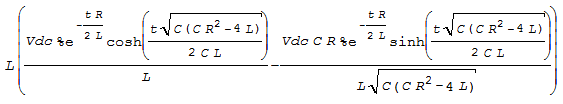
\includegraphics[scale=0.75]{./image/equacoes_1.png}
}
\end{minipage}\par
%
\item
$V_C(t)=\frac{1}{C}\int_0^ti(t)$\par
%
\begin{minipage}{0.95\linewidth}
\makebox[\linewidth]{
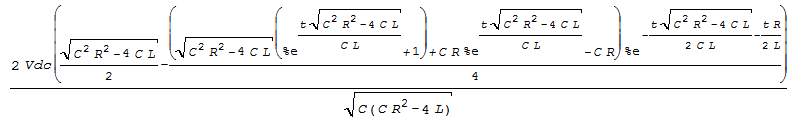
\includegraphics[scale=0.75]{./image/equacoes_2.png}
}
\end{minipage}\par
%
\end{itemize}
%enum2
\item
Para \quad $C(C R^2-4 L)=0$ \quad (Ra\'{i}zes \index{Ra\'{i}zes} iguais \index{iguais})\quad Amortecimento \index{Amortecimento} cr\'{i}tico \index{cr\'{i}tico}.\par
%
\begin{itemize}
\item
$i(t)=\frac{V_{DC}}{L} \quad  t \quad e^{\frac{-R t}{2L}} \times u(t)$\par
\item
$V_R(t)=R\times i(t)$\par
\item
$V_L(t)=L\dfrac{di(t)}{dt}$\par
%
\begin{minipage}{0.95\linewidth}
\makebox[\linewidth]{
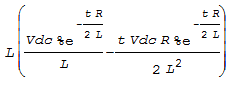
\includegraphics[scale=0.75]{./image/equacoes_3.png}
}
\end{minipage}\par
%
\item
$V_C(t)=\frac{1}{C}\int_0^ti(t)$\par
\begin{minipage}{0.95\linewidth}
\makebox[\linewidth]{
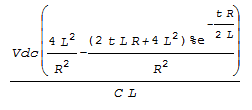
\includegraphics[scale=0.75]{./image/equacoes_4.png}
}
\end{minipage}\par
%
\end{itemize}
%enum3
\item
Para \quad $C(C R^2-4 L)<0$ \quad (Ra\'{i}zes \index{Ra\'{i}zes} complexas \index{complexas}) \quad Amortecido \index{Amortecido}.\par
%
\begin{itemize}
\item
$i(t)=\frac{2 V_{DC} C e^{\frac{-tR}{2L}} sin \left( \frac{t \sqrt{-C(CR^2-4L)}}{2CL} \right)}{\sqrt{-C(CR^2-4L)}}\times u(t)$\par
\item
$V_R(t)=R\times i(t)$\par
\item
$V_L(t)=L\dfrac{di(t)}{dt}$\par
%
\begin{minipage}{0.95\linewidth}
\makebox[\linewidth]{
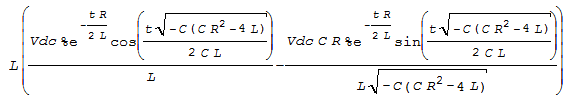
\includegraphics[scale=0.75]{./image/equacoes_5.png}
}
\end{minipage}\par
%
\item
$V_C(t)=\frac{1}{C}\int_0^ti(t)$\par
%
\begin{minipage}{0.95\linewidth}
\makebox[\linewidth]{
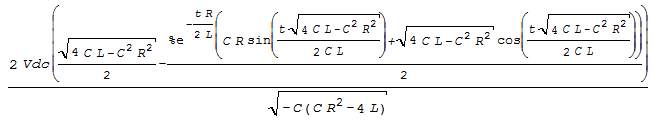
\includegraphics[scale=0.75]{./image/equacoes_6.png}
}
\end{minipage}\par
%
\end{itemize}
\end{enumerate}
%
\begin{itemize}
\item
$| \omega_n |=\sqrt{\frac{4 L-R^2 C}{4 L^2 C}}$\par
\item
%\overrightarrow{Z}
$\overline{Z}=\sqrt{R^2 + (\omega_n L -\frac{1}{\omega_n C})^2}$\par
\item
$\phi=\arctan\left(\frac{\omega_n L - \frac{1}{\omega_n C}}{R}\right)$\par
\item
$\tau=\frac{2 L}{R}$\par
\end{itemize}
%%%%%%%%%%%%%%%%%%%%%%%%%%%%%%%%%%
\begin{definition}
\begin{flalign*}
Q_c(t) =& \int^t i(t) \quad dt & \\
=& Q_c(0^-)+\int_{0^-}^t i(t) \quad dt & \\
V_c(t) =& \frac{Q_c(t)}{C} & \\
=& \frac{1}{C} \quad \int^t i_c(t) \quad dt & \\
=& \frac{Q_c(0^-)}{C} + \frac{1}{c} \quad \int_0^t i_c(t) \quad dt & \\
=& V(0^-) + \frac{1}{c} \quad \int_0^t i_c(t) \quad dt & \\
i_c(t) =& C \quad \dfrac{d V_c(t)}{dt} &
\end{flalign*}\par
\end{definition}
%
\begin{definition}
\begin{flalign*}
\psi_L(t) =& \int^t V_L(t) \quad dt & \\
=& \psi_L(0^-)+\int_{0^-}^t V_L(t) \quad dt & \\
V_L(t) =& L \quad \dfrac{d i_L(t)}{dt} & \\
i_L(t) =& \frac{\psi_L(t)}{L} & \\
=& \frac{1}{L} \quad \int^t V_L(t) \quad dt & \\
=& \frac{\psi_L(0^-)}{L} + \frac{1}{L} \quad \int_0^t V_L(t) \quad dt & \\
=& i_L(0^-) + \frac{1}{L} \quad \int_0^t V_L(t) \quad dt &
\end{flalign*}\par
\end{definition}
%
\begin{definition}
\begin{flalign*}
V_R(t) =& R \quad i_R(t) & \\
i_R(t) =& \frac{V_R(t)}{R} &
\end{flalign*}\par
\end{definition}
